\documentclass{article}
\usepackage[utf8]{inputenc}
\usepackage{graphicx}

\usepackage{xcolor}
\usepackage{listings}
\lstset{backgroundcolor=\color{lightgray},captionpos=b}
\usepackage{url}
%\usepackage[hidelinks]{hyperref}

% You must put english here to handle hyphenation correctly
% Please keep this line to avoid using the parameter from the previous article in the proceedings
%\selectlanguage{english} % possible values : french, english

\title{Dataflow tabular charts}

\author{Yves R\"utschl\'e}
%\email{yves.rutschle@apsys-airbus.com}

%\institute{APSYS}

\begin{document}
\maketitle
\index{Yves R\"utschl\'e.}
%\index{MyOtherName, A.}

\begin{abstract}
	Currently, architecture diagrams focus on network topology. This type of view does not allow a clear vision of how protocols stack up, which is important when assessing the security of a system. We propose a new type of data flow diagram which emphasizes the intertwining of multiple layers of protocols through a series of systems or security functions. These diagrams complement topological diagrams to provide a better understanding of network communications.
\end{abstract}


\section{Limits of architecture diagrams}


It is common for architecture guidelines to mention the concept of
\emph{boundary protection}. NIST Special Publication 800-53 defines\footnote{NIST.SP.800-53r4, Appendix F, SC-7.} the term as
monitoring and controling ``communications at the external boundary of the
system and at key internal boundaries within the system; implementing
subnetworks for publicly accessible system components that are separated from
internal organizational networks; and connecting to external networks or
information systems only through managed interfaces consisting of boundary
protection devices arranged in accordance with an organizational security
architecture.''

A boundary protection is more than just firewalling: the ``control'' of
communications across boundaries can be understood as application-level
filtering, or even ideally as a full protocol break.


In the definition of an architecture that relies on boundary protection,
security functions are rarely set up to create one neat barrier. Instead, they
are usually spread over various functions, each of which acts at a different
level of the network stack.

This is especially important to realize when working with architecture block
diagrams: these give a view ``from above'' of the system, where components are
laid out on the paper and the protocol stacks do not appear. This type of
representation does not readily show which processes are performed on dataflows.
For example, figure~\ref{fig:rutschle:email1} shows a standard e-mail setup: a front
firewall limits incoming dataflows to those going to the receiving SMTP server
within a DMZ; an IMAP server, still in the DMZ, accesses the files saved by the
SMTP server. A back firewall only allows IMAP connections from clients inside
the network. 

\begin{figure}[ht]
	\centering
	\includegraphics[width=1\textwidth]{img/email_above.pdf}
	\caption{Standard e-mail DMZ}
	\label{fig:rutschle:email1}
\end{figure}
% Icons from https://www.opensecurityarchitecture.org/cms/library/icon-library



The front firewall only allows traffic to the SMTP server. In case of a
vulnerability exploitation in the SMTP server, the attacker cannot move
laterally inside the network. The architect thinks they set up two security
barriers and goes home with the sense of a job well done.

This is, however, missing that the \emph{content} of the e-mail is
transmitted directly to the user e-mail client. An attacker could conceivably
use crafted headers to exploit a vulnerability in the e-mail client, and
exploit assets that are inside the protected network, beyond the back firewall.

The paranoid architect that would want to protect against that would typically
use a full protocol break, for example with a set up such as that in
figure~\ref{fig:rutschle:email2}: now the user client also runs in the DMZ,
along with a remote desktop server such as VNC or RDP, and the user connects
with a remote desktop client. Untrusted data only indirectly enters the
protected network.  Exploitation now requires a vulnerability in the SMTP or
IMAP server, to bounce and exploit a further vulnerability in the remote
desktop server.

\begin{figure}[ht]
	\centering
	\includegraphics[width=1\textwidth]{img/email_above2.pdf}
	\caption{E-mail in DMZ}
	\label{fig:rutschle:email2}
\end{figure}


However, the block diagram vision ``from above,'' both in
figure~\ref{fig:rutschle:email1} and \ref{fig:rutschle:email2}, obscures these
points, and in fact both figures look extremely similar to the hasty reader.

\section{Cutting through protocol layers}

Thus we propose the use of ``dataflow tabular charts,'' which show the network
protocol stack across the various services that the dataflow may cross. For
example figure~\ref{fig:rutschle:dtc1} shows the chart for the first architecture.

\begin{figure}[ht]
	\centering
	\includegraphics[width=1\textwidth]{img/dtc_email_simple.pdf}
	\caption{Dataflow tabular chart for E-mail in DMZ}
	\label{fig:rutschle:dtc1}
\end{figure}



Each gray box in the background represents a server, a domain, or some hardware
entity. Each vertical arrow represents an actual function or software service
and goes through the stack up to where that function processes. Then the reader
simply needs to look at what is connected to the ``Sender PC'' box to see how far
each layer can be used for attack: the original TCP connection ends at the
first firewall, but malformed SMTP can be used to attack the SMTP server; the
IMAPS server only serves files and does not read them, so it cannot be directly
attacked; the actual e-mail message reaches right through the DMZ to the final
client.

In contrast, figure~\ref{fig:rutschle:dtc2}, which shows the protocol stacks
for the second architecture, makes it clear that only the ``meaning'' of the
email (the human content) reaches the client: everything else has been
processed and re-written in the DMZ.

\begin{figure}[ht]
	\centering
	\includegraphics[width=1\textwidth]{img/dtc_email_desktop.pdf}
	\caption{Dataflow tabular chart for E-mail client in DMZ}
	\label{fig:rutschle:dtc2}
\end{figure}


These dataflow charts are meant to complete, and not replace, traditional
architectural views: while they show the processing along the network stack,
they obscure the potential for lateral movement of an attacker compromising a
vulnerable service in the DMZ. 

\section{Tooling}

We have developed and released a free software tool that can automatically
generate tabular charts from a textual representation. This approach is similar
to using \emph{GraphViz}\footnote{\url{https://www.graphviz.org/}} for oriented
graphs, or \emph{mscgen}\footnote{\url{http://www.mcternan.me.uk/mscgen/}} for
message charts: using a narrow domain-specific language along with automated
generation is the simplest way to ensure the consistency of the graphs
across a large number of figures.

The tool is available at \url{https://www.github.com/yrutschle/dtc}.

\subsection{Basic usage}


The language defines three types of entities:

\begin{description}
	\item[Systems] are drawn in the background and represent the
    physical hardware performing functions on the dataflow. An
    input line describing a system simply contains the system
    name followed by a colon:

    \begin{lstlisting}[language={},caption={System line},label={lst:rutschle:dtc_system}]
        DMZ server:
	\end{lstlisting}

\item[Functions] are typically processes that happen within a system and act on
	the dataflow. They correspond to vertical arrows in the output diagram.
	An input line describing a function is composed of:
	\verb+-> Function name (depth)+, with depth being
	the number of protocol layers that are
	processed by the function.


	Listing~\ref{lst:rutschle:dtc_function} defines three filters that cross two, three and four protocol layers respectively, resulting in figure~\ref{fig:rutschle:dtc_function}.

	\lstinputlisting[language={},
			 caption={Function line},
			 label={lst:rutschle:dtc_function}]
			 {dtc/dtc_function.dtc}
	\begin{figure}[ht]
		\centering
		\includegraphics[width=.5\textwidth]
				{img/dtc_function.pdf}
		\caption{Functions crossing protocol layers}
		\label{fig:rutschle:dtc_function}
	\end{figure}

    Note that the number of protocol layers is linked to the number of layers
    \emph{in the diagram}; this has nothing to do with OSI layers.

	\item[A protocol stack] is present between each function and contains
		the stack of protocols that these functions will use to
		exchange data. Each protocol is separated by a slash.  A
		protocol name can be left blank (e.g. if the protocol used is
		irrelevant for the diagram) or named \verb+void+ in which case the
		box won't be drawn at all (e.g. if no protocol is used for that
		layer in the current stack, but is used somewhere else. This is
		often the case when transport goes through tunnels.)

		Protocols are listed from bottom to top of the diagram and
		separated by slashes.

		Listing~\ref{lst:rutschle:dtc_stacks} shows the usage of
		\verb+void+ and blank protocols, with the resulting diagram in
		figure~\ref{fig:rutschle:dtc_stacks}. In this example, the
		physical media between the browser and the front firewall
		exists but is irrelevant, so left blank. The TLS connection
		terminates at \verb+stunnel+, and does not exist afterwards, so
		it is removed by using \verb+void+.

	\lstinputlisting[language={},
			 caption={Protocol stacks},
			 label={lst:rutschle:dtc_stacks}]
			 {dtc/dtc_stacks.dtc}
	\begin{figure}[ht]
		\centering
		\includegraphics[width=.6\textwidth]
				{img/dtc_stacks.pdf}
		\caption{Protocol stacks}
		\label{fig:rutschle:dtc_stacks}
	\end{figure}


\end{description}

One system can contain several functions, but there must always be a protocol
stack between each function, and the diagram must start and finish with a function.

A simple example where a mail client sends a mail to a mail server is shown in
listing~\ref{lst:rutschle:email2srv}. This defines a system box named `Mail
server DMZ', which contains the SMTP server and a firewall, and a `Sender PC' which contains an `Email client' function.
A data flow consisting of an e-mail message, delivered over SMTP, which is
carried over TCP over IP, is sent from the client to the server. The firewall function verifies the IP and TCP levels, so it cuts through three layers of protocols. The physical media between the e-mail client and the DMZ is unknown or irrelevant, so it is marked as \verb+void+ to keep the space empty in the protocol stack.


\lstinputlisting[language={},caption={Simple mail flow},label={lst:rutschle:email2srv}]{dtc/dtc_email2srv.dtc}



The diagram resulting from listing~\ref{lst:rutschle:email2srv} is shown in figure~\ref{fig:rutschle:email2srv}.

\begin{figure}[ht]
	\centering
	\includegraphics[width=.5\textwidth]{img/dtc_email2srv.pdf}
	\caption{Simple mail flow}
	\label{fig:rutschle:email2srv}
\end{figure}





\subsection{Improving the chart with captions}


    Each protocol can also receive a caption arrow pointing left or right,
    which is used to show where security filtering happens. These are presented
    by adding a \verb+<+ or \verb+>+ character to the left or right of the protocol name.

    Arrows can be decorated with a color that is specified with a single digit
    following the arrow sign. These colors have no defined meaning, and can be
    used to represent whatever is important for the task at hand. Possible use
    could be:
    \begin{itemize}
	    \item whether the security function is bought or home-made,
	    \item show the supplier for sets of function, by assigning a color
		    to each supplier (e.g. the diagram might be used to show
		    that two different suppliers are used on the attack path),
	    \item how effective the security function is, e.g. which EAL it is.
    \end{itemize}

    The tool currently supports five colors numbered 0 to 4: dark green, apple green, yellow, amber, and red.

    Additionally, the caption arrows are filled with references, so they can be easily commented in the text that comes with it. If left alone, the tool will simply increase a counter for each arrow. Alternatively, a reference, number or letter, can be specified in the protol stack line, after the arrow color specification. A specification such as \verb+<2,B+ will create a yellow, left-facing arrow, containing the letter `B'.

    We can then embelish our previous example to clearly document the firewall function, as shown in listing~\ref{lst:rutschle:email2srv_caption} which produces the diagram in figure~\ref{fig:rutschle:email2srv_caption}.

\lstinputlisting[language={},caption={Simple mail flow with caption arrows},label={lst:rutschle:email2srv_caption}]{dtc/dtc_email2srv_caption.dtc}


\begin{figure}[ht]
	\centering
	\includegraphics[width=.5\textwidth]{img/dtc_email2srv_caption.pdf}
	\caption{The firewall prevents outgoing TCP/IP connections (1 and 2), and checks incoming connections (3 and A)}
	\label{fig:rutschle:email2srv_caption}
\end{figure}


\subsection{Adding icons}

A security function can also be represented by an icon on the function arrow. This is done by adding a file name, along with the protocol levels, in brackets, following the function definition. For example we can add a firewall icon to the IP layer of our example, along with an envelope at the e-mail level, as shown in listing~\ref{lst:rutschle:email2srv_icons} and figure~\ref{fig:rutschle:email2srv_icons}.

\lstinputlisting[language={},caption={Simple mail flow with icons},label={lst:rutschle:email2srv_icons}]{dtc/dtc_email2srv_icons.dtc}



    
\begin{figure}[ht]
	\centering
	\includegraphics[width=.5\textwidth]{img/dtc_email2srv_icons.pdf}
	\caption{Chart with function icon}
	\label{fig:rutschle:email2srv_icons}
\end{figure}


    
\subsection{Generating the chart}

Once the input text is written, generating the chart as SVG is as simple as:

    \begin{lstlisting}[language={},caption={Running DTC},label={lst:rutschle:dtc_run}]
        dtc.pl input.dtc
    \end{lstlisting}

    which will generate a `.svg' file. For RFC lovers, it is also possible
    to specify the output format as text using \verb+--format text+, which
    results in beautiful ASCII output as shown in
    figure~\ref{fig:rutschle:rfc}.

\begin{figure}[ht]
	\centering
	\includegraphics[width=.5\textwidth]{img/rfc.pdf}
	\caption{Dataflow tabular chart for RFC editors}
	\label{fig:rutschle:rfc}
\end{figure}


\section{Future works}

As with all software project, \emph{dtc} is a work in progress and several areas of improvement are already known. In particular:

\begin{itemize}
	\item The input parser is not very robust, and may fail upon finding incorrect description files.
	\item Text that is too long will not overflow gracefully; additional flexibility, or at the very least warnings, should be added.
	\item There is no test suite.
	\item Colors and general appearance of the diagrams are not very configurable. Graphical elements could be marked with CSS to provide for easy external configuration so the user can pick colors, fonts and so on.
	\item Unified diagrams that combine topological information and protocol information may be invented, for example based on isometric 3D.
	\item Currently the tool is quite static and requires writing descriptions specifically for each diagram.  Integration with architecture modeling tool may provide ways to automatically create diagrams from a central model.
\end{itemize}

% TODO

% - look into standardized DSLs if someone asked the same questions to prevent "one more standard" approaches => Interface with modeling tools?
% - find a hybrid representation with architecture and protocol data => isometric 3D?
% - style sheets for colors and fonts, better color support
% - Integration of text with LaTeX?
% - Make parser more robust

\section{Conclusion}

We have presented a new type of diagram to clearly represent the layering of network protocols. These diagrams can be used alongside topological architecture diagrams to provide a better overall understanding of complex systems.
\end{document}
